\documentclass[a4paper,12pt]{article}

\usepackage{amsmath}
\usepackage{graphicx}
\usepackage[margin=20mm]{geometry}
\usepackage[colorlinks=true]{hyperref}
\urlstyle{same}
\usepackage{lineno}
\renewcommand\linenumberfont{\normalfont\tiny}
%\linenumbers
\usepackage{wrapfig}
\usepackage{subcaption}
\usepackage{authblk}
\usepackage{booktabs}
\usepackage{pstricks}
\usepackage{pstricks-add}

\title{The Study of the Silicon Detector Response for p-Carbon Polarization Measurements at RHIC}

\author[1]{D.~Smirnov\thanks{d.s@plexoos.com}}
\author[2]{D.~Kalinkin}
\author[]{\ldots}

\affil[1]{Brookhaven National Lab}	
\affil[2]{ITEP}

\begin{document}

\maketitle

\begin{abstract}
At RHIC the measurements of proton beam polarization are carried out
by inserting a carbon target in the beam, and regestering the scattered carbon
ions with silicon detectors. In this note we present the results of the
analysis of the silicon detectors response to carbon atoms and alpha particles.
\end{abstract}

\section{Motivation and Measurement Principles}

During the 2013 run we observed significant changes in the gain in some of the
silicon detectors. The detector gain was monitored by taking calibration runs
when there was no beam in the machine. We use two radioactive source emmiting
alpha particles at known energies.

\section{Results}

\subsection{Calibration}

Some calorimetry is done by measuring amplitudes and integrals of the signals
from the silicon detector. In order to convert these values from ADC counts
to the energy scale units we need to obtain properties of our calibration
curve i.e. calibrate. One of the possible calibration procedures is alpha
calibration. The idea is to put low intensity fixed energy alpha source
somewhere in acceptance region of the detector and then look for the corresponding
peak in the distribution of particles by ADC bins. Alpha source energy and
position of this peak give us fixed point on the calibration curve.

At the moment, two polarimeters (Y1D and B1U) has only a single americium source
($E_{\text{Am}} = 5486.0\text{ MeV}$), while other two (Y2U and B2D) has also additional
gadolinium source ($E_{\text{Gd}} = 3271.21\text{ MeV}$). Before now only americium point was
used, the relation between americium energy $E_{\text{Am}}$ and peak position $\mu_{\text{Am}}$
was called americium gain. Conversion from ADC counts were performed by multiplying by this value.

Information about gadolinium peak can tell us more about our calibration curve.
For instance we can take gadolinium gain and linear two-point (americium and gadolinium) fit slope
 and compare them to americium gain (Fig.~\ref{fig:gain_relations}).

\begin{figure}[p]
\begin{subfigure}[b]{0.5\textwidth}
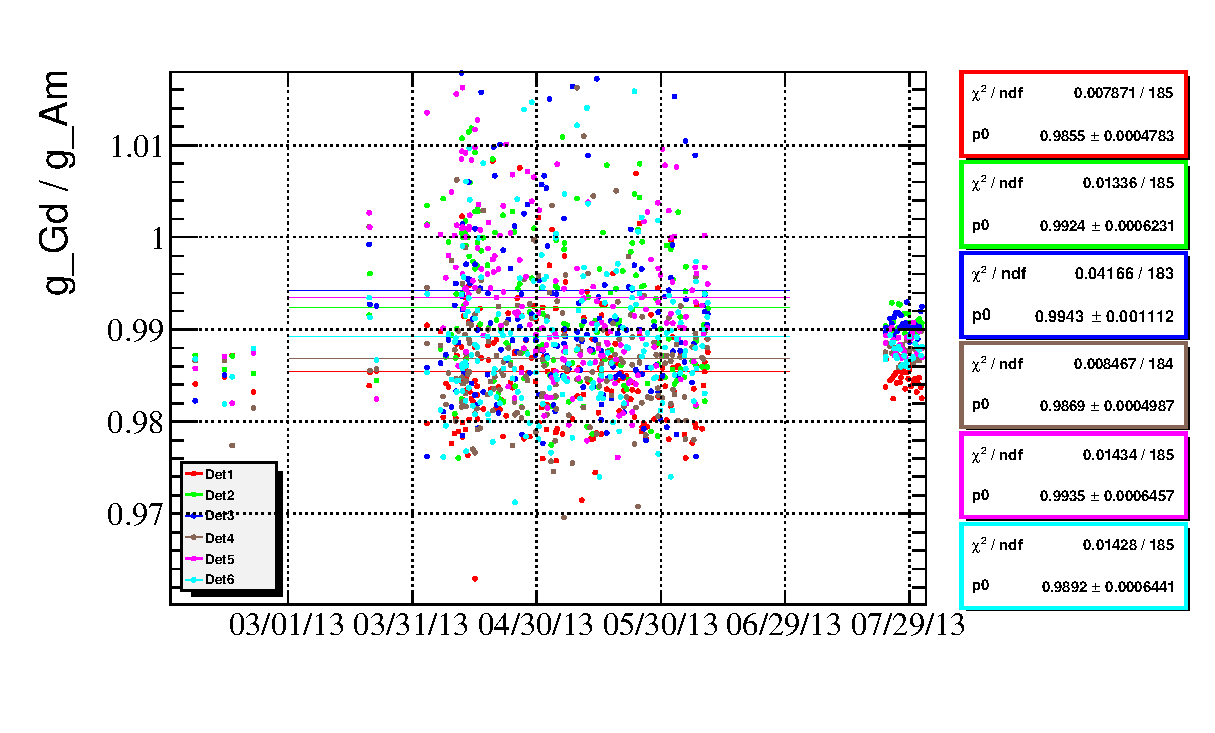
\includegraphics[width=\textwidth]{gfx/run13_alpha_study/Y2U/c_chGdGain_over_AmGain_by_day_Y2U.eps}
\caption{Relation of gadolinium and americium gains}
\end{subfigure}
\begin{subfigure}[b]{0.5\textwidth}
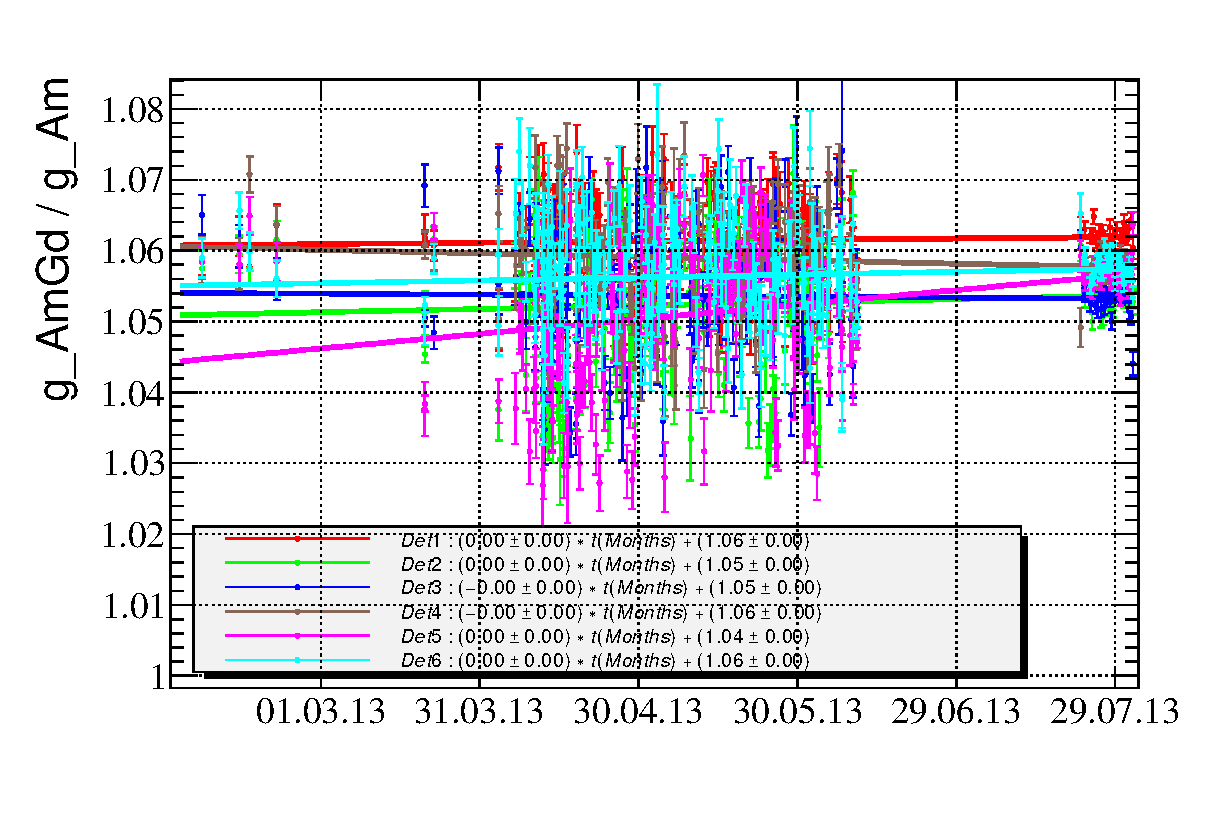
\includegraphics[width=\textwidth]{gfx/run13_alpha_study/Y2U/c_chAmGdGain_over_AmGain_by_day_Y2U.eps}
\caption{Relation of two-point (americium and gadolinium) linear fit slope and americium gain}
\end{subfigure}
\caption{Comparison of different approaches to gain calculation (data for Y2D polarimeter).
Cut to remove outliers was applied to this plot.}
\label{fig:gain_relations}
\end{figure}

\subsection{Atten}

There are several stages of amplification of the detector signal. Some checks
for linearity of this amplification can be done by inserting attenuators in
different places of the signal path. Shaper motherboard has resistive divider
with a multiplexer which is controlled by software. During alpha measurement
this attenuator is switched to state $1/5$. Alpha peaks can be seen using
different possible attenuator settings, which allows us to test stuff.
Resulting distributions can be seen on (Fig.~\ref{fig:atten_distrib})

\begin{table}[htb]
\caption{The mean positions of the Am and Gd alpha peaks at different attenuator settings.}
\centering

\begin{tabular}{clrr}
\toprule
Atten   &       Run ID & AmPeakPos      & GdPeakPos \\
\midrule
$\frac{1}{10}$  & \small{atten\_1\_over\_10.yel2.alpha0}        & $77.0\pm0.7$          & $44.2\pm0.4$ \\
\addlinespace
$\frac{1}{5}$   & \small{13\_310713.yel2.alpha0}                & $154.9\pm2.7$         & $88.9\pm1.5$ \\
\addlinespace
$\frac{1}{3}$   & \small{atten\_1\_over\_3.yel2.alpha0}         & ---\hspace{20pt}      & $149.4\pm2.5$ \\
\bottomrule
\end{tabular}

\label{table:atten}
\end{table}

Then relative non-linearity values are

\begin{equation}
\frac{154.9}{77.0 \times 2} - 1 = 0.6\%
\qquad
\frac{88.9}{44.0 \times 2} - 1 = 0.6\%
\qquad
\frac{149.4*3}{88.9 \times 5} - 1 = 0.8\%
\end{equation}

They are small enough.

\begin{figure}[p]
\begin{subfigure}[b]{0.3\textwidth}
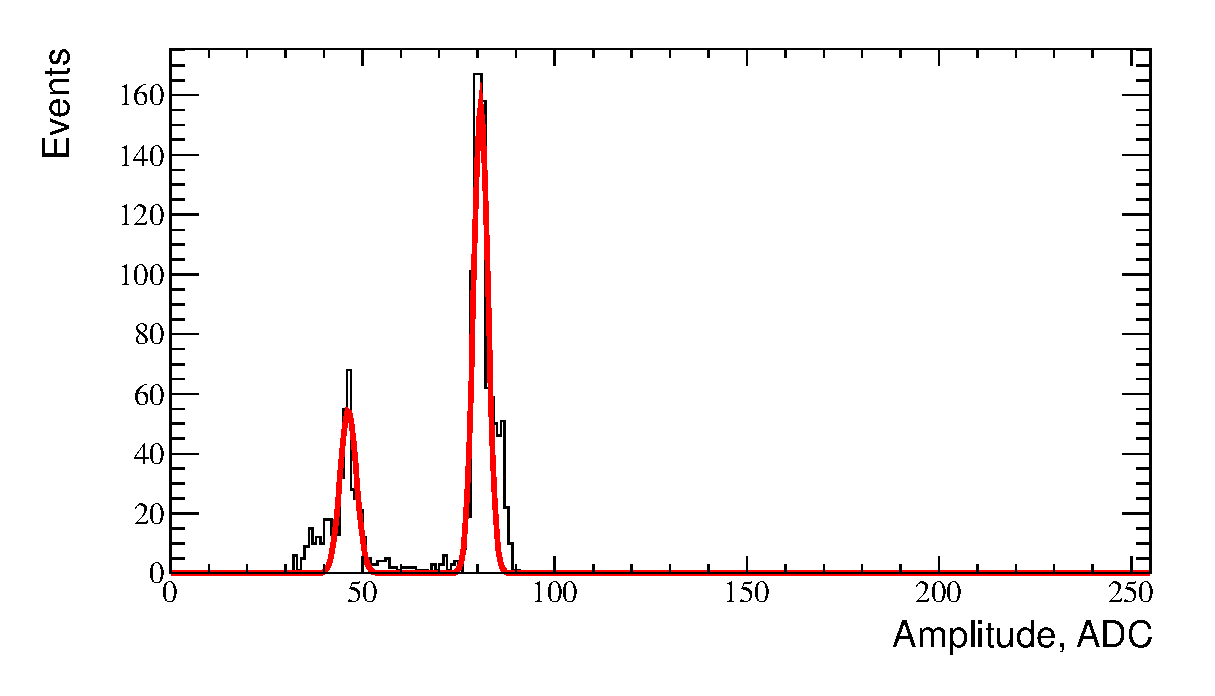
\includegraphics[width=\textwidth]{gfx/atten_1_over_10_ch06.eps}
\caption{$\text{attenuator}=1/10$}
\end{subfigure}
\begin{subfigure}[b]{0.3\textwidth}
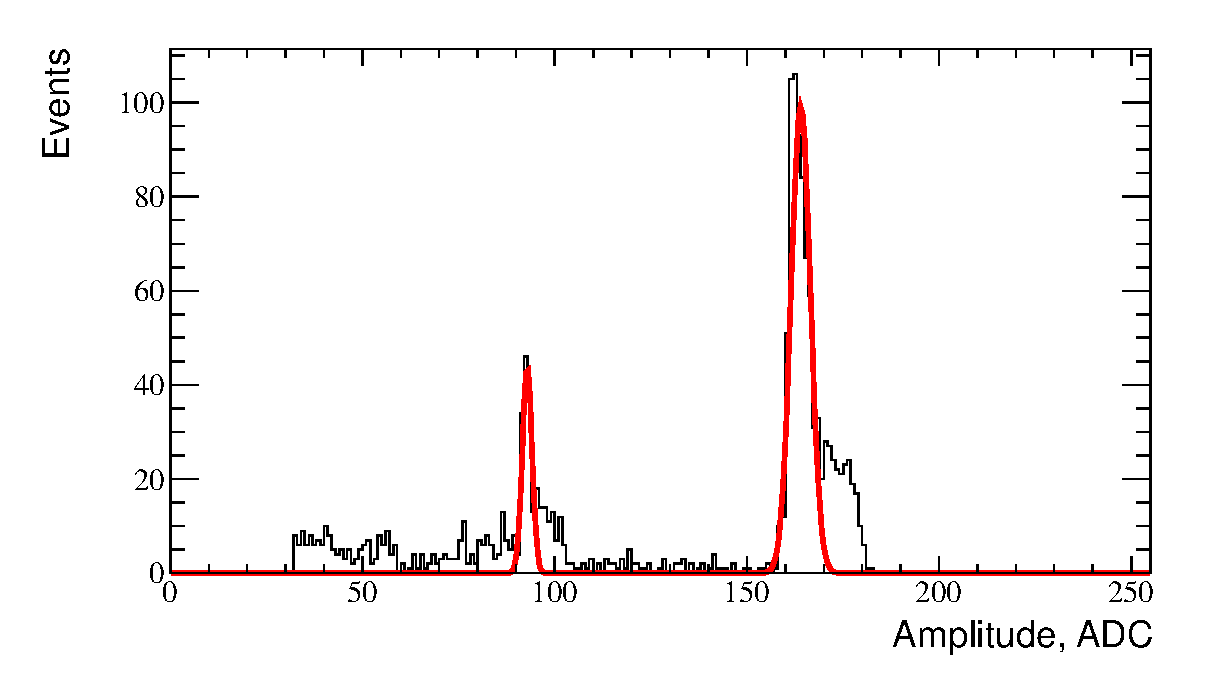
\includegraphics[width=\textwidth]{gfx/atten_1_over_5_ch06.eps}
\caption{$\text{attenuator}=1/5$}
\end{subfigure}
\begin{subfigure}[b]{0.3\textwidth}
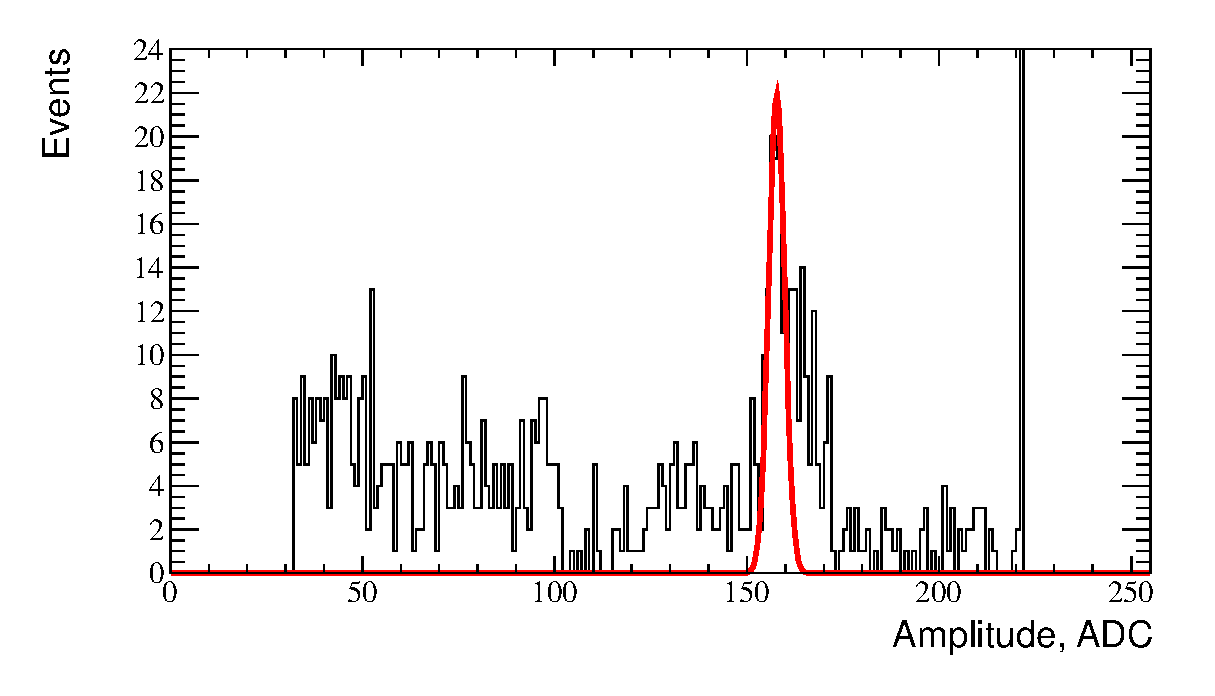
\includegraphics[width=\textwidth]{gfx/atten_1_over_3_ch06.eps}
\caption{$\text{attenuator}=1/3$}
\end{subfigure}
\caption{Alpha peaks seen with different onboard attenuator settings (Y2U)}
\label{fig:atten_distrib}
\end{figure}

\subsection{Dead layer size}

\begin{wrapfigure}{r}{0.3\textwidth}
\vspace{-30pt}
\begin{center}
\setlength{\unitlength}{0.035\textwidth}
\psset{unit=\unitlength}

\begin{pspicture}(0,0)(10,10) % for debugging add [showgrid=true]

% yaxe
\psStartPoint(0.4,0)\psVector(0,10)
\rput[r](0,10){ADC}

% xaxe
\psStartPoint(0,0.4)\psVector(10,0)
\rput[t](10,0){E}

% adc americium tick
\psline(0.2,7)(0.6,7)
\rput[r](0,7){$\mu_\text{Am}$}

% adc gadolinium tick
\psline(0.2,4)(0.6,4)
\rput[r](0,4){$\mu_\text{Gd}$}

\psline(2,0)(8,8)

\psline(2.3,0.2)(2.3,0.6)
\rput[lt](2.3,0){$E_\text{DL}$}

\psline(5,0.2)(5,0.6)
\rput[t](5,0){$E_\text{Gd}$}

\psline(7.2,0.2)(7.2,0.6)
\rput[t](7.2,0){$E_\text{Am}$}

\end{pspicture}

\end{center}
\caption{Linear approximation calibraion curve}
\label{fig:calib_curve}
\end{wrapfigure}

Our model for silicon detector assumes that there is a layer where our detector has
zero response as a calorimeter -- dead layer. Adding gadolinium alpha source to the
setup allows us to put one more calibration point on our callibration curve. Using
americium and gadolinium points we can estimate thickness of this layer.

Intersection of linear fit with energy axis gives us approximation to energy
deposited by alpha particles in dead layer.
Assuming that local gain values for both calibration points are equal we can write:

\begin{equation}
\frac{\mu_{Am}}{E_{Am} - E_{DLAm}} = \frac{\mu_{Gd}}{E_{Gd} - E_{DLGd}},
\label{eq:gain_equality}
\end{equation}

\noindent where $\mu$ -- measured ADC counts, $E$ -- alpha source energy value.
Stopping power for 5 MeV and 3 MeV alpha particles is different. Meanwhile
particle passing through dead layer doesn't loose enough energy to let
stopping power change. Thus giving us linear dependency for the loss energy.

\begin{equation}
E_{DLAm} \simeq x_{DL} \lambda_{Am}\qquad
E_{DLGd} \simeq x_{DL} \lambda_{Gd}\qquad
\label{eq:linear_loss}
\end{equation}

\noindent Combining (\ref{eq:gain_equality}) and (\ref{eq:linear_loss}) we obtain following formula
for dead layer size:

\begin{equation}
x_{DL} = \frac{\mu_{Gd} E_{Am} - \mu_{Am} E_{Gd}}{\mu_{Gd}\lambda_{Am} - \mu_{Am}\lambda_{Gd}}
\label{eq:x_dl}
\end{equation}

\begin{figure}[p]
\begin{subfigure}[b]{0.5\textwidth}
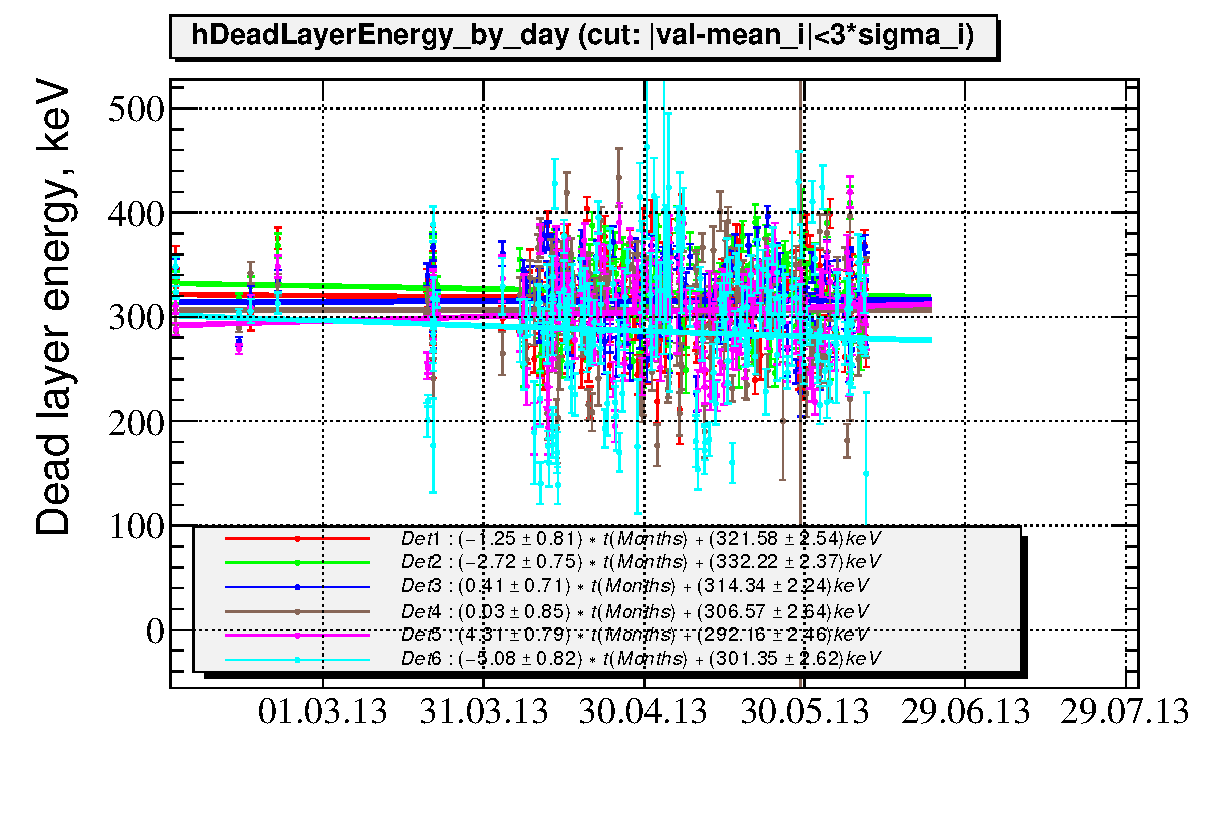
\includegraphics[width=\textwidth]{gfx/run13_alpha_study/B2D/c_chDeadLayerEnergy_by_day_B2D.eps}
\caption{B2D}
\end{subfigure}
\begin{subfigure}[b]{0.5\textwidth}
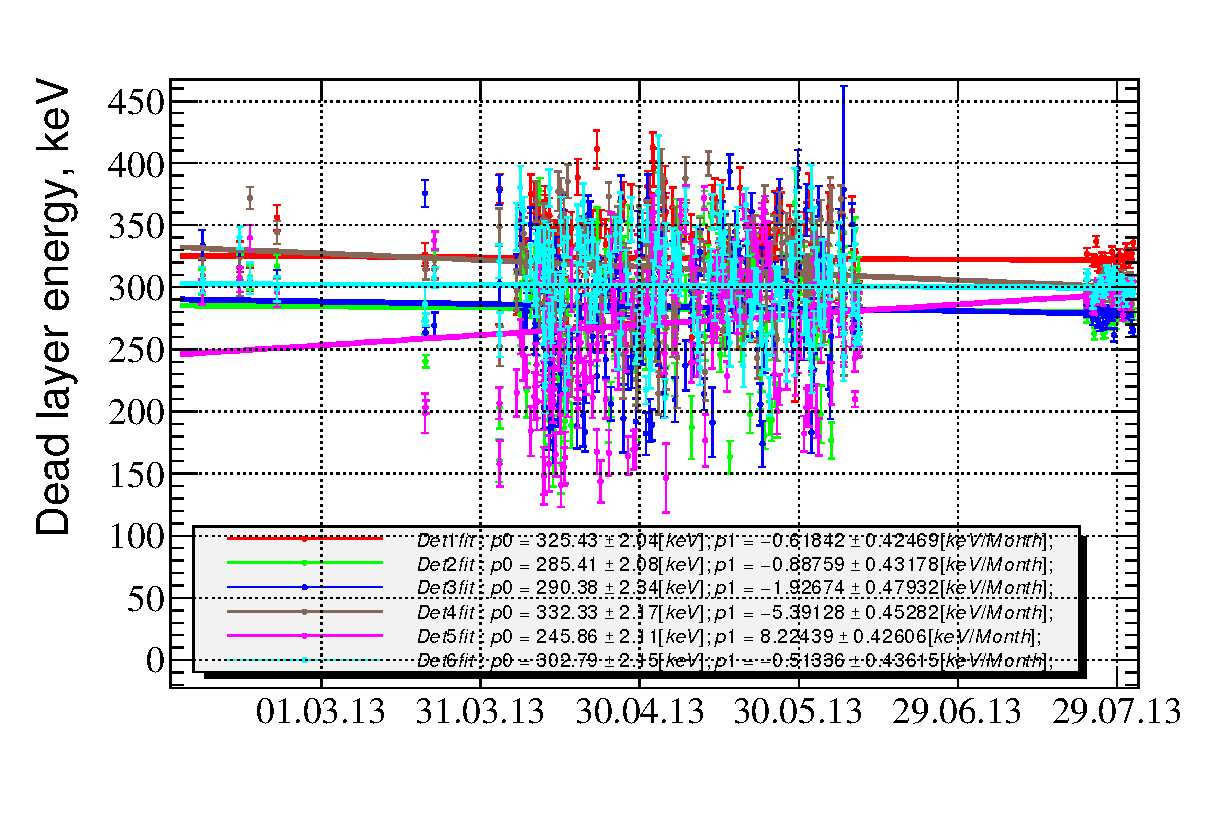
\includegraphics[width=\textwidth]{gfx/run13_alpha_study/Y2U/c_chDeadLayerEnergy_by_day_Y2U.eps}
\caption{Y2U}
\end{subfigure}
\caption{$E_{DL}$ (see \ref{fig:calib_curve}) is the missing energy value extracted from linear fit
of the americium and gadolinium points. Cut to remove outliers was applied to this plot.}
\label{fig:e_dl}
\end{figure}

\begin{figure}[p]
\begin{subfigure}[b]{0.5\textwidth}
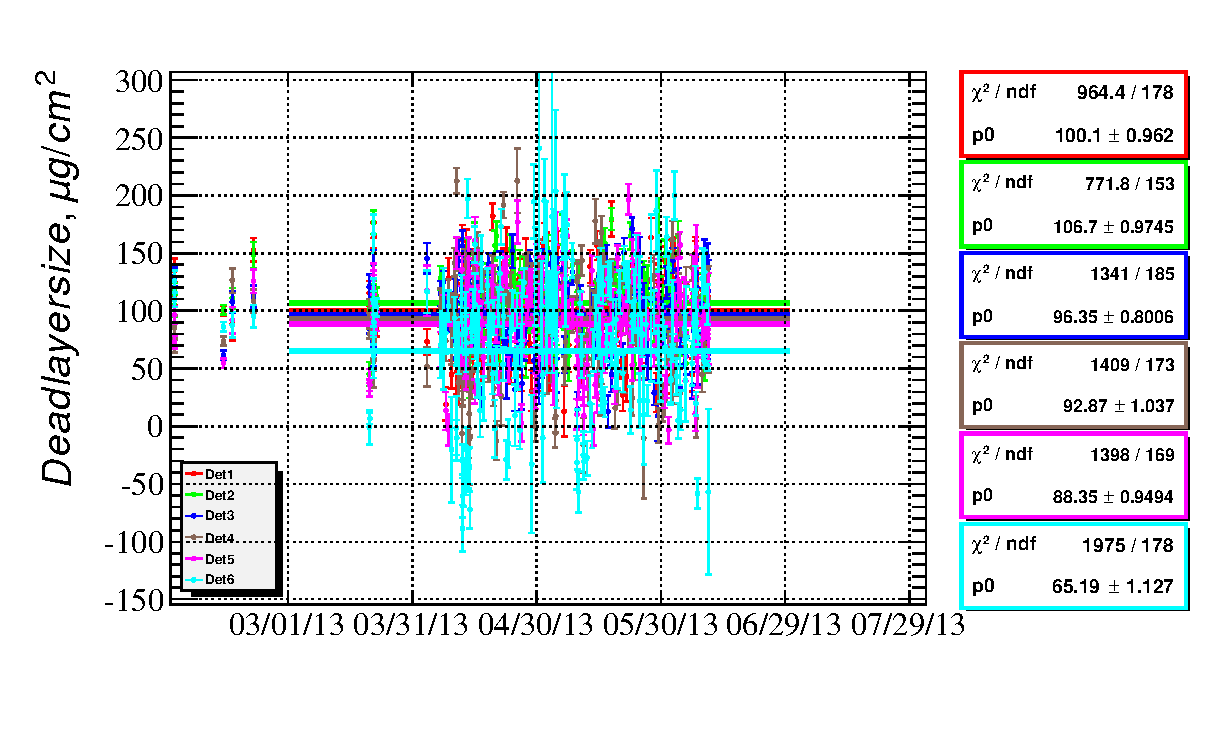
\includegraphics[width=\textwidth]{gfx/run13_alpha_study/B2D/c_chDeadLayerSize_by_day_B2D.eps}
\caption{B2D}
\end{subfigure}
\begin{subfigure}[b]{0.5\textwidth}
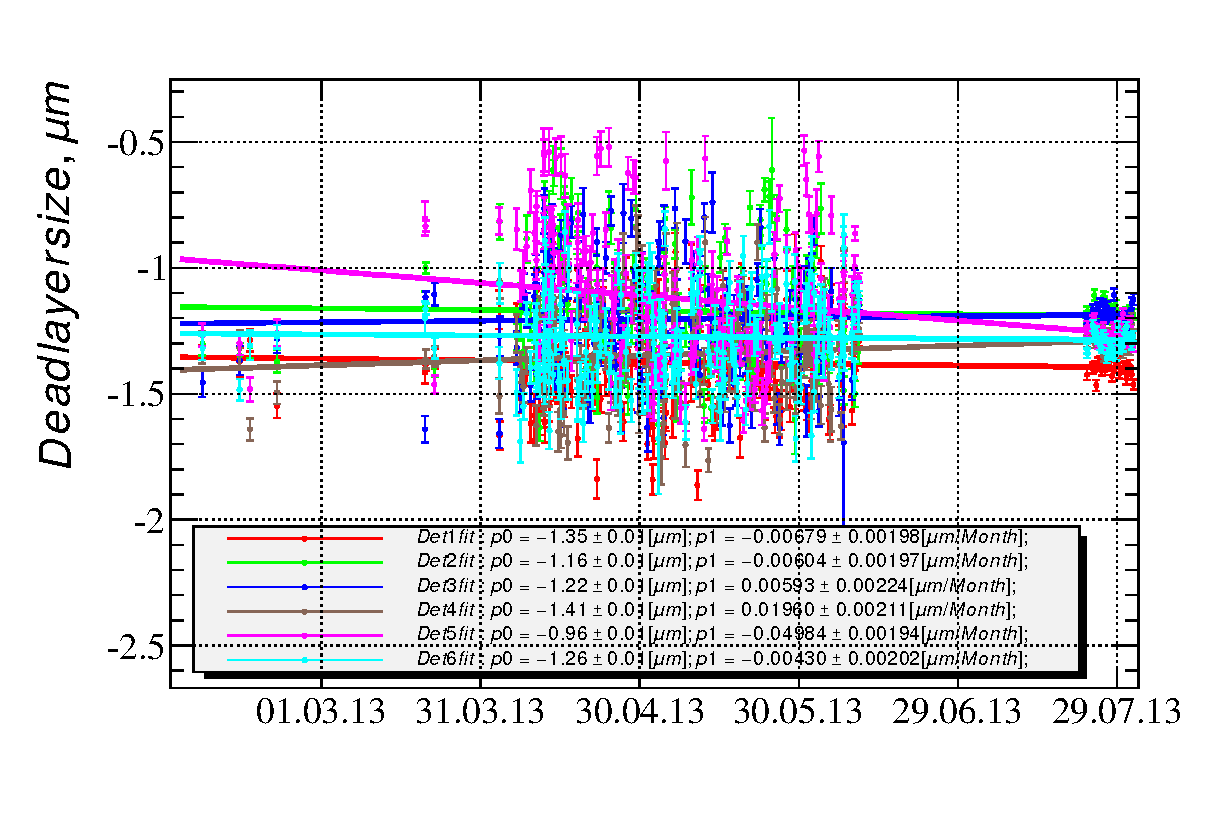
\includegraphics[width=\textwidth]{gfx/run13_alpha_study/Y2U/c_chDeadLayerSize_by_day_Y2U.eps}
\caption{Y2U}
\end{subfigure}
\caption{$x_{DL}$ is the dead layer thickness calculated using formula (\ref{eq:x_dl}). Cut to remove
outliers was applied to this plot.}
\label{fig:x_dl}
\end{figure}

\subsection{Bias current}

% TODO: write something about how out bias current varies over time

On figures~\ref{fig:gain_relations},\ref{fig:e_dl} and \ref{fig:x_dl} there are few measurements
before and after the beam session showing much lower spread. This looks to be a result of some
parameter variation due to beam pickup.

One of the work parameters of our silicon detector that we measure is a bias current -- current
constantly flowing through detector (in this case -- set of 12 strips). Current was measured
for each of the six silicon detectors on all polarimeters, measurements were taken each five
minutes. Values lie mostly in range from $-30$ to $0$~$\mu A$. It was interesting to see how
this current affects calibration characteristics of our detector. For example, it is known 
that higher bias voltage should decrease size of depleted zone, i.e. decrease size of dead layer.
On our plots (Fig.~\ref{fig:bc_vs_xdl}) we see some weak correlation between dead layer size and bias
current.

\begin{figure}[p]
\begin{subfigure}[b]{0.5\textwidth}
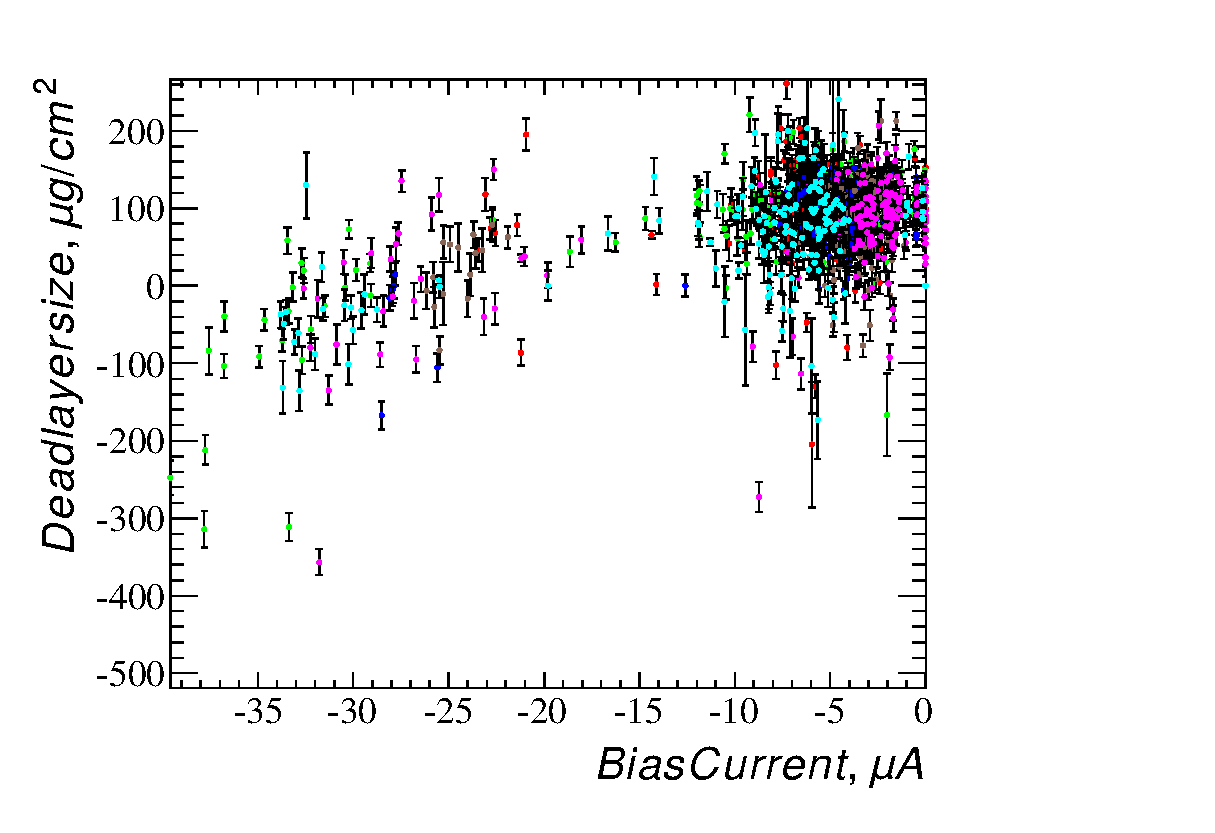
\includegraphics[width=\textwidth]{gfx/run13_alpha_study/B2D/c_hBiasCurrent_DeadLayerSize.eps}
\caption{B2D}
\end{subfigure}
\begin{subfigure}[b]{0.5\textwidth}
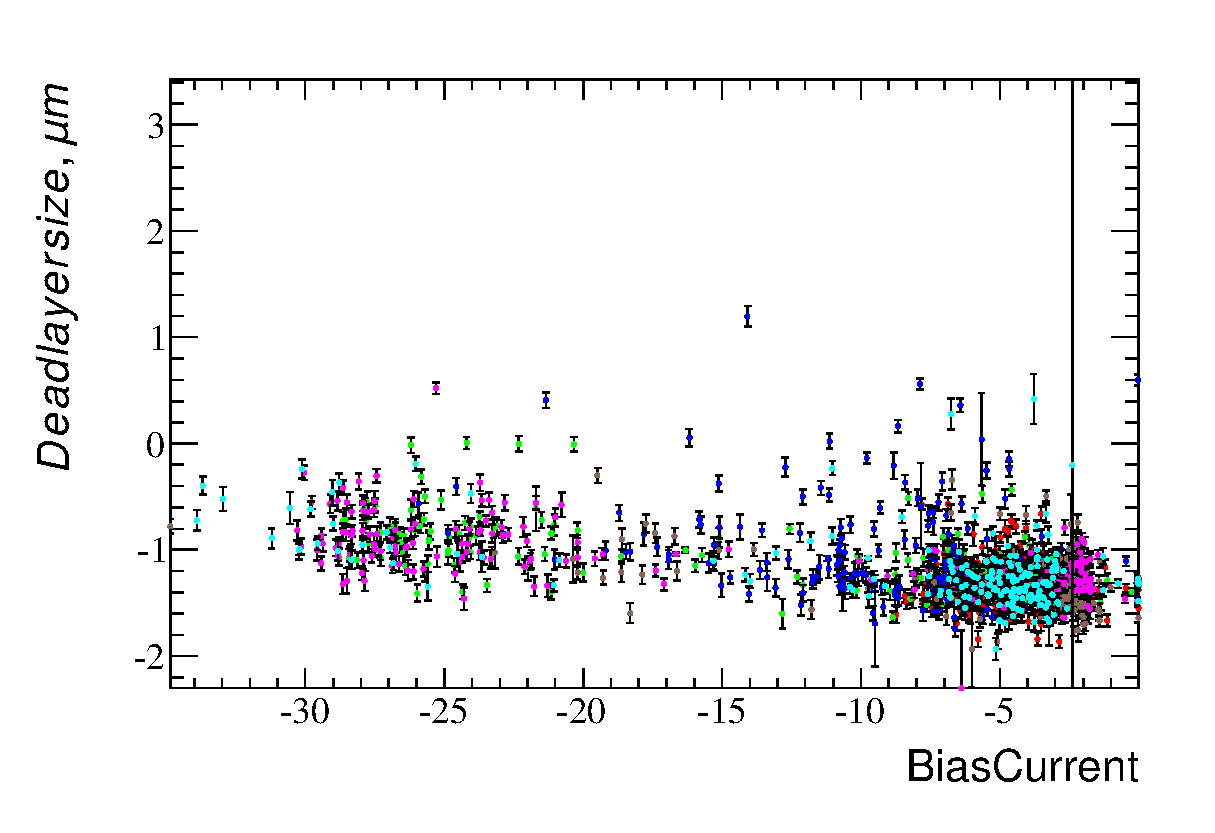
\includegraphics[width=\textwidth]{gfx/run13_alpha_study/Y2U/c_hBiasCurrent_DeadLayerSize.eps}
\caption{Y2U}
\end{subfigure}
\caption{Bias current versus dead layer size dependency}
\label{fig:bc_vs_xdl}
\end{figure}

Much stronger correlation is seen when we compare bias current with gain (Fig.~\ref{fig:bc_vs_gain}).
Bias current during polarization measurement can differ from the bias current in the time of
alpha measurement, so correction to gain value should be applied.

Additional correlation seen on plots \ref{bc_vs_gain-b1u} and \ref{bc_vs_gain-y1d} corresponds to
special set of measurements with varied bias voltage.

\begin{figure}[p]
\begin{subfigure}[b]{0.5\textwidth}
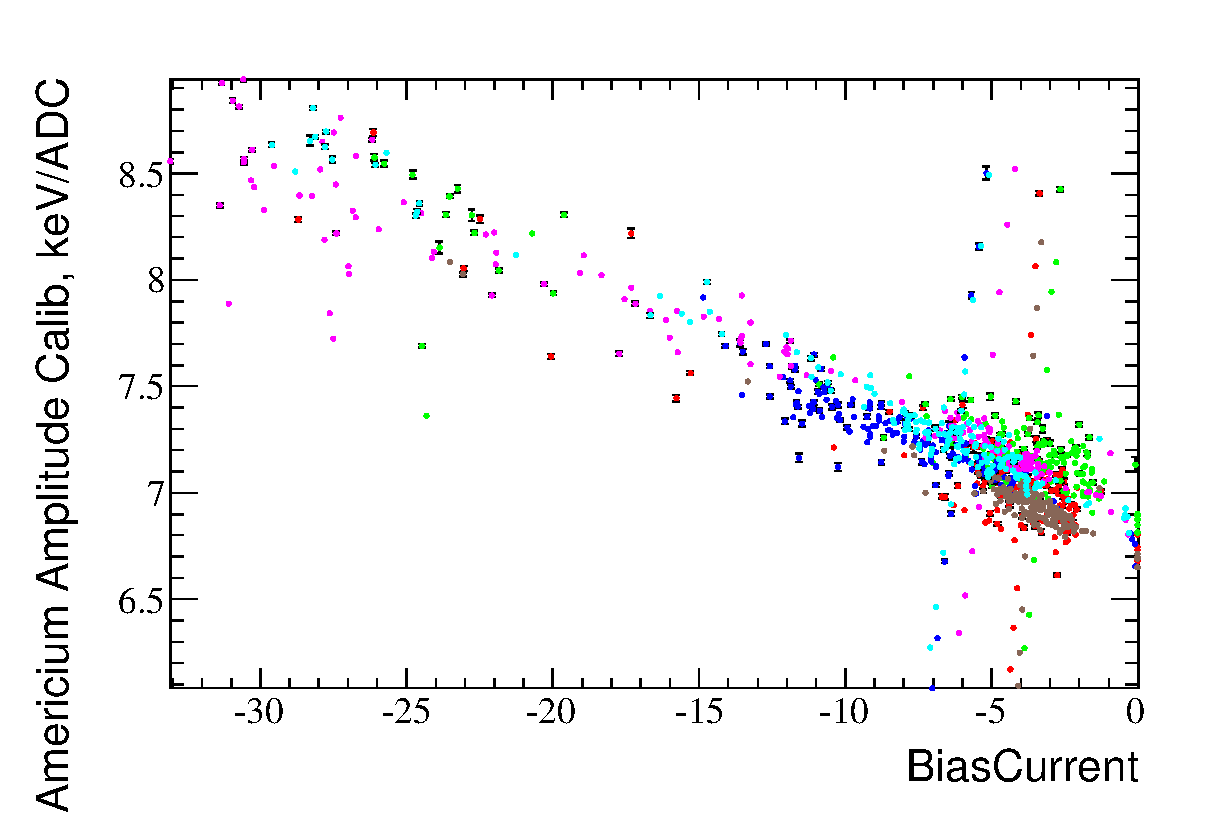
\includegraphics[width=\textwidth]{gfx/run13_alpha_study/B1U/c_hBiasCurrent_AmAmpCoef.eps}
\caption{B1U}\label{bc_vs_gain-b1u}
\end{subfigure}
\begin{subfigure}[b]{0.5\textwidth}
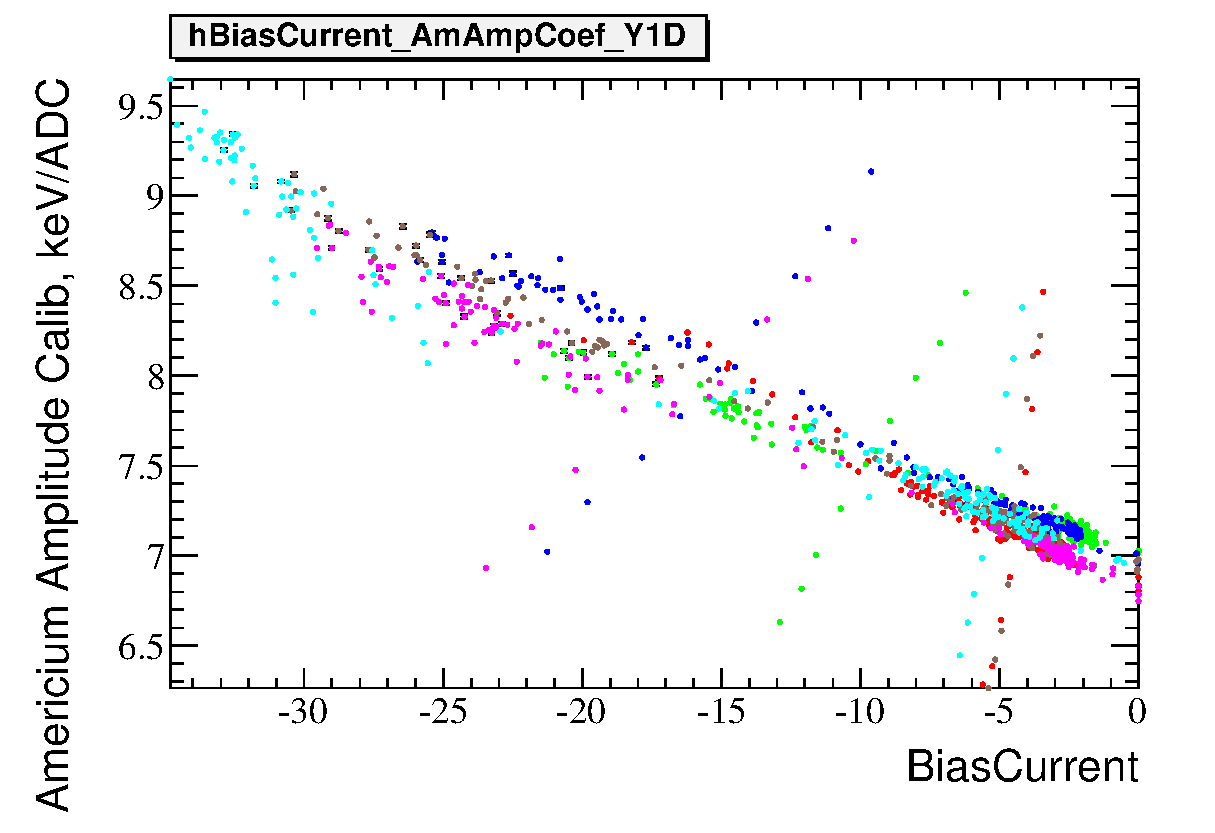
\includegraphics[width=\textwidth]{gfx/run13_alpha_study/Y1D/c_hBiasCurrent_AmAmpCoef.eps}
\caption{Y1D}\label{bc_vs_gain-y1d}
\end{subfigure}

\begin{subfigure}[b]{0.5\textwidth}
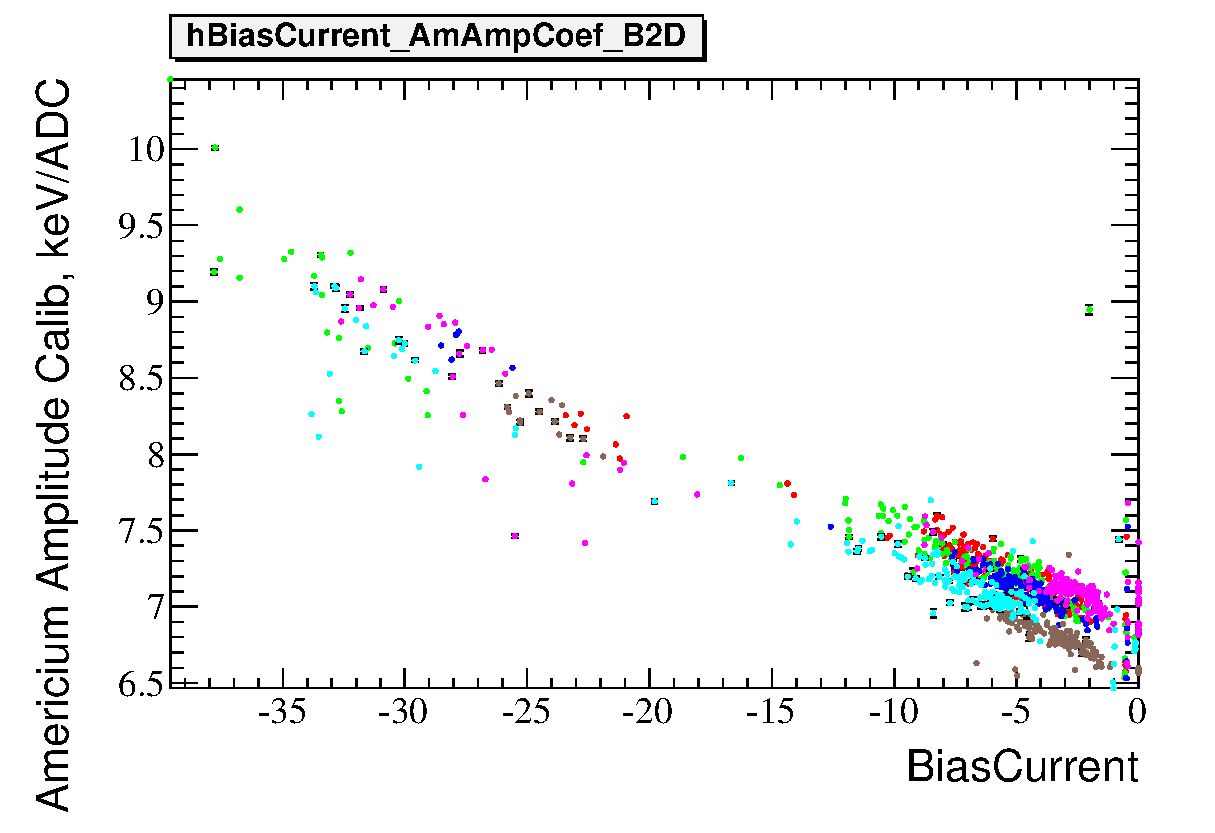
\includegraphics[width=\textwidth]{gfx/run13_alpha_study/B2D/c_hBiasCurrent_AmAmpCoef.eps}
\caption{B2D}\label{bc_vs_gain-b2d}
\end{subfigure}
\begin{subfigure}[b]{0.5\textwidth}
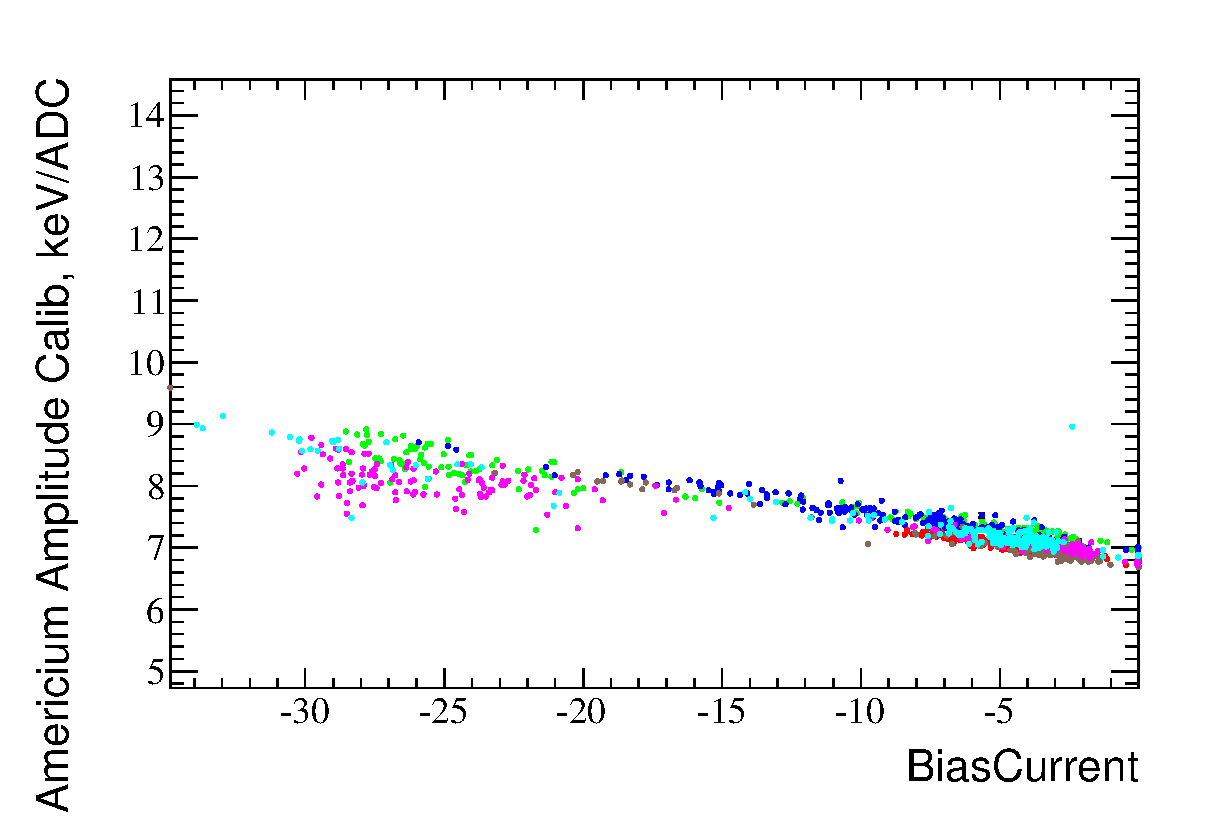
\includegraphics[width=\textwidth]{gfx/run13_alpha_study/Y2U/c_hBiasCurrent_AmAmpCoef.eps}
\caption{Y2U}\label{bc_vs_gain-y2u}
\end{subfigure}

\caption{Bias current versus americium gain ($E_{\text{Am}} / \mu_{\text{Am}}$) dependency}
\label{fig:bc_vs_gain}
\end{figure}

\begin{figure}[p]
\begin{subfigure}[b]{0.5\textwidth}
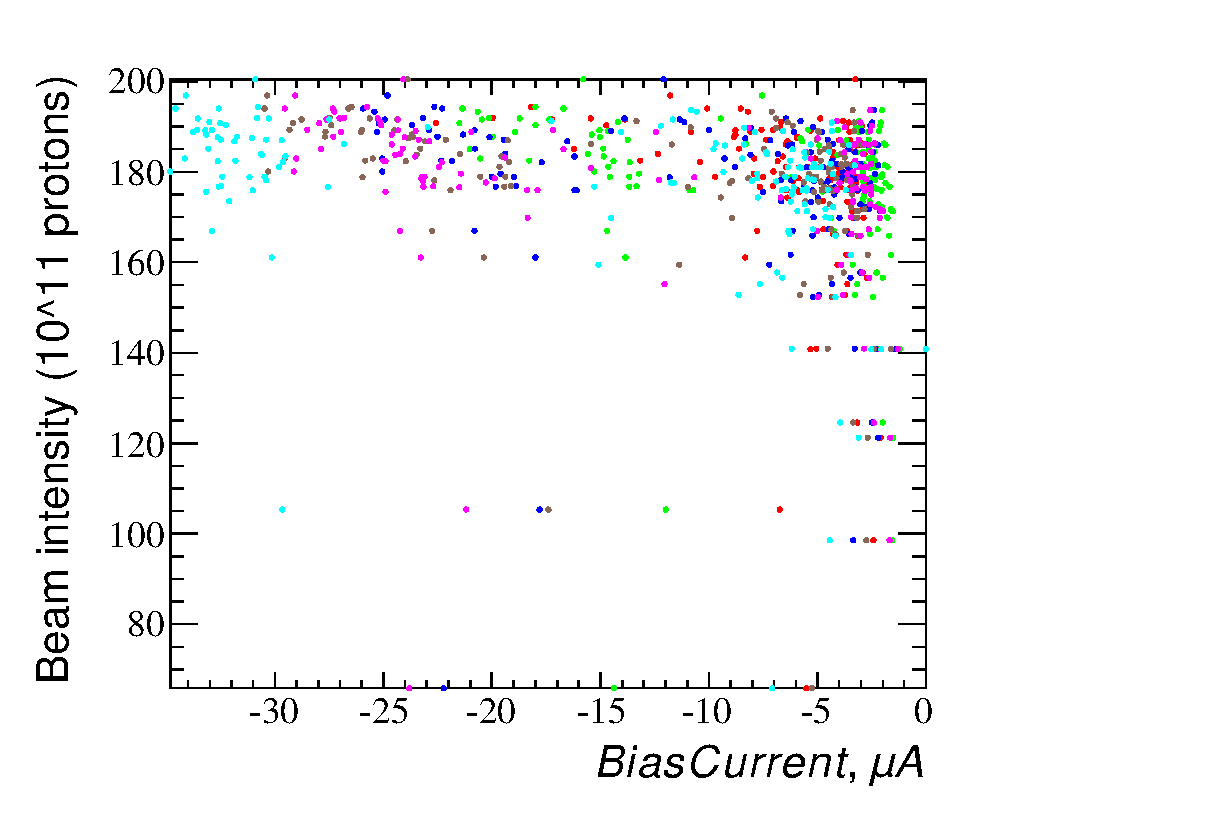
\includegraphics[width=\textwidth]{gfx/run13_alpha_study/Y1D/c_hBiasCurrent_BeamCurrent.eps}
\caption{Y1D}
\end{subfigure}
\begin{subfigure}[b]{0.5\textwidth}
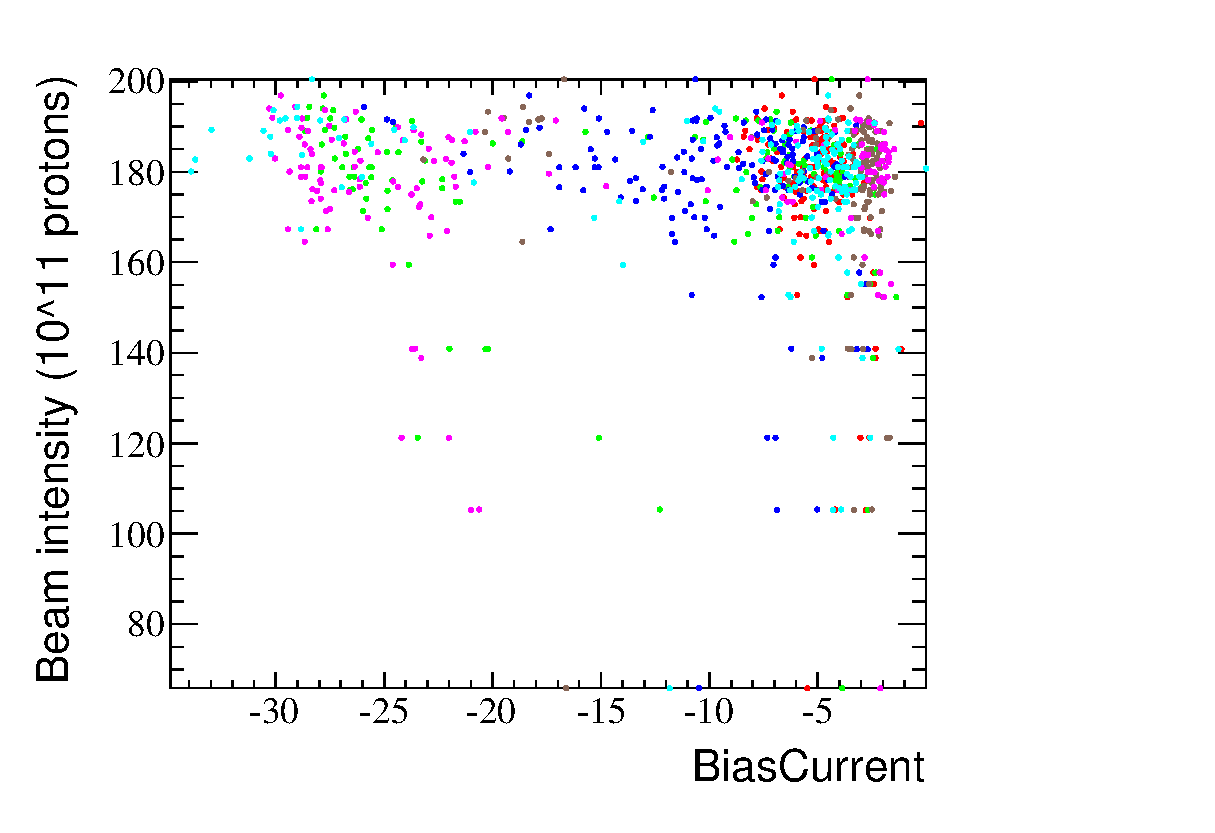
\includegraphics[width=\textwidth]{gfx/run13_alpha_study/Y2U/c_hBiasCurrent_BeamCurrent.eps}
\caption{Y2U}
\end{subfigure}
\caption{Bias current during alpha measurement versus beam current during the fill.}
\end{figure}

\section{Conclusions}

\end{document}
